%% abtex2-modelo-relatorio-tecnico.tex, v-1.7.1 laurocesar
%% Copyright 2012-2013 by abnTeX2 group at http://abntex2.googlecode.com/ 
%%
%% This work may be distributed and/or modified under the
%% conditions of the LaTeX Project Public License, either version 1.3
%% of this license or (at your option) any later version.
%% The latest version of this license is in
%%   http://www.latex-project.org/lppl.txt
%% and version 1.3 or later is part of all distributions of LaTeX
%% version 2005/12/01 or later.
%%
%% This work has the LPPL maintenance status `maintained'.
%% 
%% The Current Maintainer of this work is the abnTeX2 team, led
%% by Lauro César Araujo. Further information are available on 
%% http://abntex2.googlecode.com/
%%
%% This work consists of the files abntex2-modelo-relatorio-tecnico.tex,
%% abntex2-modelo-include-comandos and abntex2-modelo-references.bib
%%

% ------------------------------------------------------------------------
% ------------------------------------------------------------------------
% abnTeX2: Modelo de Relatório Técnico/Acadêmico em conformidade com 
% ABNT NBR 10719:2011 Informação e documentação - Relatório técnico e/ou
% científico - Apresentação
% ------------------------------------------------------------------------ 
% ------------------------------------------------------------------------

% Alterado por Rodrigo Campiolo para apresentação de relatórios na disciplina
% de Redes de Computadores II do Bacharelado em Ciência da Computação da UTFPR-CM.


\documentclass[
	% -- opções da classe memoir --
	12pt,				% tamanho da fonte
	%openright,			% capítulos começam em pág ímpar (insere página vazia caso preciso)
	oneside,   	        % para impressão em verso e anverso use twoside. Oposto a oneside
	a4paper,			% tamanho do papel. 
	% -- opções da classe abntex2 --
	%chapter=TITLE,		% títulos de capítulos convertidos em letras maiúsculas
	%section=TITLE,		% títulos de seções convertidos em letras maiúsculas
	%subsection=TITLE,	% títulos de subseções convertidos em letras maiúsculas
	%subsubsection=TITLE,% títulos de subsubseções convertidos em letras maiúsculas
	% -- opções do pacote babel --
	english,			% idioma adicional para hifenização
	french,				% idioma adicional para hifenização
	spanish,			% idioma adicional para hifenização
	brazil,				% o último idioma é o principal do documento
	]{pacotes/abntex2}


% ---
% PACOTES
% ---

% ---
% Pacotes fundamentais 
% ---
\usepackage{cmap}				% Mapear caracteres especiais no PDF
\usepackage{lmodern}			% Usa a fonte Latin Modern
\usepackage[T1]{fontenc}		% Selecao de codigos de fonte.
\usepackage[utf8]{inputenc}		% Codificacao do documento (conversão automática dos acentos)
\usepackage{indentfirst}		% Indenta o primeiro parágrafo de cada seção.
\usepackage{algorithm}      % Escrever algoritmos
\usepackage{algpseudocode}      % Escrever algoritmos
\usepackage{color}				% Controle das cores
\usepackage{graphicx}			% Inclusão de gráficos
\usepackage{hyperref}           % Links
\usepackage{listings}           % Comandos
\usepackage{pgfplots}           % Comandos
% ---

% ---
% Pacotes adicionais, usados no anexo do modelo de folha de identificação
% ---
\usepackage{multicol}
\usepackage{multirow}
% ---
	
% ---
% Pacotes adicionais, usados apenas no âmbito do Modelo Canônico do abnteX2
% ---
\usepackage{lipsum}				% para geração de dummy text
% ---

% ---
% Pacotes de citações
% ---
\usepackage[brazilian,hyperpageref]{backref}	 % Paginas com as citações na bibl
\usepackage[alf]{pacotes/abntex2cite}	% Citações padrão ABNT

% --- 
% CONFIGURAÇÕES DE PACOTES
% --- 

% ---
% Configurações do pacote backref
% Usado sem a opção hyperpageref de backref
\renewcommand{\backrefpagesname}{Citado na(s) página(s):~}
% Texto padrão antes do número das páginas
\renewcommand{\backref}{}
% Define os textos da citação
\renewcommand*{\backrefalt}[4]{
	\ifcase #1 %
		Nenhuma citação no texto.%
	\or
		Citado na página #2.%
	\else
		Citado #1 vezes nas páginas #2.%
	\fi}%
% ---

% ---
% Informações de dados para CAPA e FOLHA DE ROSTO
% ---
\titulo{Análise empírica de\\ algoritmos de subarranjo máximo}
\autor{Alexandre Yuji Kajihara\\Clodoaldo Basaglia da Fonseca}
\local{Campo Mourão}
\data{Junho / 2017}
\instituicao{%
  Universidade Tecnológica Federal do Paraná -- UTFPR
  \par
  Departamento Acadêmico de Computação -- DACOM
  \par
  Bacharelado em Ciência da Computação -- BCC
}
\tipotrabalho{Relatório técnico}
% O preambulo deve conter o tipo do trabalho, o objetivo, 
% o nome da instituição e a área de concentração 
\preambulo{Relatório técnico de atividade prática solicitado pelo professor Rodrigo Campiolo na disciplina de Análise de Algoritmos do Bacharelado em Ciência da Computação da Universidade Tecnológica Federal do Paraná.}
% ---

% ---
% Configurações de aparência do PDF final

% alterando o aspecto da cor azul
\definecolor{blue}{RGB}{41,5,195}

% informações do PDF
\makeatletter
\hypersetup{
     	%pagebackref=true,
		pdftitle={\@title}, 
		pdfauthor={\@author},
    	pdfsubject={\imprimirpreambulo},
	    pdfcreator={LaTeX with abnTeX2},
		pdfkeywords={abnt}{latex}{abntex}{abntex2}{relatório técnico}, 
		colorlinks=true,       		% false: boxed links; true: colored links
    	linkcolor=blue,          	% color of internal links
    	citecolor=blue,        		% color of links to bibliography
    	filecolor=magenta,      		% color of file links
		urlcolor=blue,
		bookmarksdepth=4
}
\makeatother
% --- 

% --- 
% Espaçamentos entre linhas e parágrafos 
% --- 

% O tamanho do parágrafo é dado por:
\setlength{\parindent}{1.3cm}

% Controle do espaçamento entre um parágrafo e outro:
\setlength{\parskip}{0.2cm}  % tente também \onelineskip

% ---
% compila o indice
% ---
\makeindex
% ---

% Omite a numeração de capítulos
\renewcommand*\thesection{\arabic{section}}



% ----
% Início do documento
% ----
\begin{document}

% Retira espaço extra obsoleto entre as frases.
\frenchspacing 

% ----------------------------------------------------------
% ELEMENTOS PRÉ-TEXTUAIS
% ----------------------------------------------------------
% \pretextual

% ---
% Capa
% ---
%\imprimircapa
% ---

% ---
% Folha de rosto
% (o * indica que haverá a ficha bibliográfica)
% ---
\imprimirfolhaderosto
% ---


% ---
% RESUMO
% ---

% resumo na língua vernácula (obrigatório)
\begin{resumo}
A análise empírica é uma maneira de verificar a execução de diferentes algoritmos, que tem o mesmo objetivo e conferir qual deles apresenta uma melhor performance.Um problema que apresenta algumas formas de se implementar é o problema subarranjo máximo, que dada uma sequência de valores, tentar encontrar os valores que tem o maior valor de soma. Com quatro das várias maneiras existentes de se implementar esse algoritmo, utilizamos a linguagem de programação \textif{Swift}, na qual implementamos os algoritmos medindo o tempo de cada um deles. A nossa entrada foi um arranjo de valores negativos e positivos gerados aleatoriamente, na qual foram utilizados os mesmos em todos os algoritmos. Conseguimos obter sucesso em todos os tamanhos de vetores que propomos e foi visível a diferença de um algoritmo para outro que tem o mesmo objetivo.

\vspace{\onelineskip}
    
 \noindent
\textbf{Palavras-chave}: análise de algoritmos. \textit{Swift},análise empirica.
\end{resumo}
% ---

% ---
% inserir lista de ilustrações
% ---
%\pdfbookmark[0]{\listfigurename}{lof}
%\listoffigures*
%\cleardoublepage
% ---

% ---
% inserir lista de tabelas
% ---
%\pdfbookmark[0]{\listtablename}{lot}
%\listoftables*
%\cleardoublepage
% ---

% ---
% inserir lista de abreviaturas e siglas
% ---
%\begin{siglas}
%  \item[IP] Internet Protocol
%  \item[TCP] Transmission Control Protocol
%  \item[UDP] User Datagram Protocol
%\end{siglas}
% ---

% ---
% inserir o sumario
% ---
\pdfbookmark[0]{\contentsname}{toc}
\tableofcontents*
\cleardoublepage
% ---

% ----------------------------------------------------------
% ELEMENTOS TEXTUAIS
% ----------------------------------------------------------
\textual

\makeatletter
\renewcommand{\chapter}{\@gobbletwo}
\makeatother

\section{Introdução}
\label{sec:introducao}
A análise empírica também é importante na comparação de dois algoritmos que podem ou podem não tem a mesma ordem de complexidade \cite{Sanders:2002}.

Devido a existência do problema do subarranjo máximo, que de acordo Kamran Ashraf dado uma sequência de valores A= \{$a_1$, $a_2$, ..., $a_n$\}, nós iremos tentar encontrar a subsequência de A contínua a qual os valores tem a maior soma \cite{Ashraf:2015}. Dito isso, foi implementando quatro algoritmos que resolvem esse problema, em que um deles envolvem três iterações aninhadas, e o outro uma versão melhorada desse algoritmo anterior.

Uma das soluções para esse problema é a divisão e conqusita que consiste em: a instância dada do problema é dividida em duas ou mais instâncias menores, cada instância menor é resolvida usando o próprio algoritmo que está sendo definido, as soluções das instâncias menores são combinadas para produzir uma solução da instância original \cite{DC:Feofiloff:2013}.

A última solução para esse problema é a de programação dinâmica: é uma espécie de tradução iterativa inteligente da recursão e pode ser definido, vagamente, como "recursão com apoio de uma tabela" \cite{PD:Feofiloff:2013}.

Para a resolução dese problema e para comparação desse algoritmos, utilizamos a linguagem de programação \textit{Swift}. O trabalho aqui apresentado está organizado da seguinte forma: na seção \ref{sec:objetivos} é apresentado o objetivo desse trabalho do estudo, ou seja, mensurar o tempo de diferentes algoritmos que tem o mesmo propósito; na seção \ref{sec:fundamentacao} são apresentadas as fundamentações que seriam o que foi necessário para realização desse trabalho; na seção \ref{sec:materiais} é descrito os materiais que foram utilizados; na seção \ref{sec:procedimentos} os procedimentos e resultados que foram obtidos após executar os quatro algoritmos; na seção \ref{sec:discussao} a disussão dos resultados que foram conquistados; na seção \ref{sec:conclusoes} a conclusão após realizar esse trabalho; e por fim na seção \ref{sec:referencias} as referências utilizadas.

\section{Objetivos}
\label{sec:objetivos}
O objetivo desse trabalho é realizar a análise empírica de quatro algoritmos que utilizam conceitos diferentes para resolução do problema do subarranjo máximo. As entradas foram de tamanhos diferentes, na qual foram escolhido um arranjo com tamanho de 10, 100, 1000 e 10000, e os valores presentes em cada uma dessas posições são diferentes. Após executar três vezes para cada um desses tamanhos, foi tirado uma média de tempo em milisegundos, que irá ser apresentando na seção \ref{sec:discussao}.

\section{Fundamentação}
\label{sec:fundamentacao}
Os fundamentos necessários nesse trabalho foram basicamente, a instalação da linguagem de programação \textit{Swift}. Primeiramente devemos fazer o \textit{download} do \textit{Swift} pelo terminal mesmo em que podemos utilizar o seguinte comando:


\begin{lstlisting}[language=bash]
  $ wget https://swift.org/builds/swift-3.1.1-release/ubuntu1610/swift-3.1.1-RELEASE/swift-3.1.1-RELEASE-ubuntu16.10.tar.gz
\end{lstlisting}

na qual escolhemos o \textit{Swift} 3.1.1 para o Ubuntu 16.10, que foi o Sistema Operacional utilizado e ser a última versão até o momento da realização desse trabalho. Após isso, podemos extraír o arquivo realizando o seguinte comando:

\begin{lstlisting}[language=bash]
  $ tar -xf swift-3.1.1-RELEASE-ubuntu16.10
\end{lstlisting}

Com arquivo extraído teremos que fazer uma alteração em um arquivo presente em nosso sistema que é o \textit{~./profile}, que pode ser acessado da seguinte maneira:

\begin{lstlisting}[language=bash]
  $ sudo nano ~/.profile
\end{lstlisting}

Você pode utilizar outros editores vi, gedit, xed, Atom,etc. Na última linha desse arquivo iremos adicionar a linha abaixo. Isso é necessário para que não tenhamos que executar toda vez que ligarmos nossa máquina esse comando, em que devemos passar o lugar onde foi extraído aquele arquivo que realizamos o \textit{download} que no meu caso foi no Documentos.

\begin{lstlisting}[language=bash]
  export PATH=~/Documentos/swift-3.1.1-RELEASE-ubuntu16.10/usr/bin/:"{\$PATH}"
\end{lstlisting}

Agora podemos executar o comando abaixo para ver as opções fornecidas pela linguagem:

\begin{lstlisting}[language=bash]
  swift --help
\end{lstlisting}

Em alguns casos pode ser necessário a instalação do clang, que pode ser instalado da seguinte maneira: 

\begin{lstlisting}[language=bash]
  sudo apt-get install clang
\end{lstlisting}

Enfim, podemos escrever códigos na linguagem de programação \textit{Swift}, em que para compilar podemos utilizar o seguinte comando:

\begin{lstlisting}[language=bash]
  swiftc name-file.swift
\end{lstlisting}

em que no nosso caso compilamos dá seguinte maneira: 

\begin{lstlisting}[language=bash]
  swiftc main.swift algoritmo.swift
\end{lstlisting}

No nosso caso para evitar de ter que escrever todo esse comando para compilar utilizamos o Makefile, que pode ser instalado: 

\begin{lstlisting}[language=bash]
    sudo apt-get install make
\end{lstlisting}

Para evitar tudo de digitar, podemos dar os dois seguinte comandos:

\begin{lstlisting}[language=bash]
    make all 
\end{lstlisting}

\begin{lstlisting}[language=bash]
    make
\end{lstlisting}

caso queira remover o arquivo executável, é só digitar: 

\begin{lstlisting}[language=bash]
    make clear
\end{lstlisting}

Por fim, para executar o nosso programa é só utilizarmos o comando:

\begin{lstlisting}[language=bash]
    ./main
\end{lstlisting}

\section{Materiais}
\label{sec:materiais}
Os materiais necessários foram um caderno, lápis, um \textit{laptop} com as seguintes configurações:
\begin{itemize}
    \item Sistema Operacional Ubuntu 16.10 64 bits    
    \item Intel Core i7-6500U
    \item 16 GB de memória RAM (\textit{Random Access Memory})
    \item \textit{Swift} na versão 3.1.1 
    \item Editor de textoSublime Text Build 3126
\end{itemize}

\section{Procedimentos e Resultados}
\label{sec:procedimentos}
Os procedimentos necessários para realizar a análise empírica dos algoritmos que resolvem o problema do subarranjo máximo foi a instalação do \textit{Swift} na qual citamos na seção \ref{sec:fundamentacao}. 

Após isso, escrevemos o nosso código-fonte. Antes de implementar os quatros algoritmos, criamos dois arranjos unidimensionais de inteiros. O primeiro subarranjo preenchemos com valores, que começam com o metade do tamanho do vetor multiplicado por menos um. Com esses valores incrementamos um a cada vez que se alterava de posição. Exemplo: se o tamanho do nosso arranjo é 100, na posição zero do vetor irá estar o valor -50, na posição 1, o valor -49, na posição dois o valor -48, e assim por diante, até que todos as posições estejam preenchidas, como podemos ver no algoritmo \ref{algo:preencheprimeiroarranjo}. Com o primeiro arranjo preenchido, iremos preencher o segundo, em que geramos um valor no intervalo de zero até o tamanho do primeiro arranjo, e pegamos o valor que está na posição gerada aleatória e adicionamos no segundo arranjo. Removemos esse valor do primeiro arranjo e repetimos esse processo até preencher o segundo arranjo, isso nos garante que não tenhamos valores repetidos e que tenhamos valores negativos, essa função pode ser vista no algoritmo  \ref{algo:preenchesegundoarranjo}.

Para fins de testes rápidos, foram comentados em meio ao código, vetores já preenxidos com deferentes tamanhos. Para utilizá-los, basta seguir as instruções que seguem comentadas junto a eles.

\begin{algorithm}
\caption{Algoritmo que preenche o primeiro arranjo}
\label{algo:preencheprimeiroarranjo}
\begin{algorithmic}[1]
    \Function{geraVetor}{$valores$, $n$}
        \State  $i = 0$
        \State  $valor = (n / 2) * (-1)$
        \While{$i < n$}
            \State $valores[i] = valor$ 
            \State $valor = valor + 1$
            \State $i = i + 1$
        \EndWhile
        \State \Return
    \EndFunction
\end{algorithmic}
\end{algorithm}

\begin{algorithm}
\caption{Algoritmo que preenche o segundo arranjo}
\label{algo:preenchesegundoarranjo}
\begin{algorithmic}[1]
    \Function{preencheVetor}{$valores, vetor, n$}
        \State  $i = 0$
        \State  $valor = (n / 2) * (-1)$
        \While{$i < n$}
            \State $posicao = (random()\%valores.length)$
            \State $vetor[i] = valores[posicao]$
            \State $remove(valores[posicao])$
            \State $i = i + 1$
        \EndWhile
        \State \Return
    \EndFunction
\end{algorithmic}
\end{algorithm}

Após termos o nosso arranjo com valores aleatórios iremos aplicar os mesmos em funções que tentam resolver o subarranjo máximo. O primeiro algoritmo é chamado de \textit{enumeration()} utilizando três iterações aninhadas, para tentar achar o valor, como pode ser visto no algoritmo  \ref{algo:enumeration}. 

\begin{algorithm}[!htb]
\caption{Algoritmo \textit{enumeration()}}
\label{algo:enumeration}
\begin{algorithmic}[1]
    \Function{enumeration}{$vetor, n$}
        \State  $i = 0, j = 0, k = 0$
        \State  $somatorio = 0, melhor = 0$
        \While{$i < n$}
            \State $j = i$
            \While{$j < n$}
                \State $somatorio = 0$
                \State $k = i$
                \While{$k < j$}
                    \State $somatorio = somatorio + vetor[k]$ 
                    \State $k = k + 1$
                \EndWhile
                \If{$somatorio > melhor$}
                    \State  $melhor = somatorio$
                \EndIf
                \State $j = j + 1$
            \EndWhile
            \State $i = i + 1$
        \EndWhile
        \State \Return $melhor$
    \EndFunction
\end{algorithmic}
\end{algorithm}

Feito o algoritmo \ref{algo:enumeration} utilizamos a mesma idéia para realizar o segundo quese trata de  uma melhoria do primeiro. Uma de suas diferenças que podemos notar é um laço aninhados a menos, do que em relação ao algoritmo \ref{algo:enumeration}, o segundo algoritmo pode ser visto \ref{algo:betterEnumeration}. 

\begin{algorithm}[!htb]
\caption{Algoritmo \textit{betterEnumeration()}}
\label{algo:betterEnumeration}
\begin{algorithmic}[1]
    \Function{betterEnumeration}{$vetor, n$}
        \State  $i = 0, j = 0$
        \State  $somatorio = 0, melhor = 0$
        \While{$i < n$}
            \State $somatorio = 0$
            \State $j = i$
            \While{$j < n$}
                \State $somatorio = somatorio + vetor[j] $
                \If{$somatorio > melhor$}
                    \State  $melhor = somatorio$
                \EndIf
                \State $j = j + 1$
            \EndWhile
            \State $i = i + 1$
        \EndWhile
        \State \Return $melhor$
    \EndFunction
\end{algorithmic}
\end{algorithm}

O penúltimo algoritmo utilizado foi dito em seções anteriores, utilizam o conceito de divisão e conquista. Basicamente ele divide o arranjo em metade e vai calculando o somatório de cada uma dessas metades, e por fim verifica qual subarranjo possui o máximo valor, em que iremos apresentar logo abaixo o algoritmo \ref{algo:divideAndConquer}.

\begin{algorithm}[!htb]
\caption{Algoritmo \textit{divideAndConquer()}}
\label{algo:divideAndConquer}
\begin{algorithmic}[1]
    \Function{divideAndConquer}{$vetor, inicio, fim$}
        \If{$inicio > fim$}
            \State \Return $0$
        \EndIf
        \If{$inicio == fim$}
           \State \Return $max(0, vetor[inicio])$
        \EndIf
        \State  $meio = (inicio+fim) / 2$
        \State  $maiorEsquerda = 0$
        \State  $somatorio = 0$
        \State  $i = meio$
        \While{$i >= inicio$}
            \State $somatorio = somatorio + vetor[i] $
            \If{$somatorio > maiorEsquerda$}
                \State $maiorEsquerda = somatorio$
            \EndIf
            \State $i = i - 1$
        \EndWhile
        \State  $maiorDireita = 0$
        \State  $somatorio = 0$
        \State  $i = meio + 1$
        \While{$i <= fim$}
            \State $somatorio = somatorio + vetor[i] $
            \If{$somatorio > maiorDireita$}
                \State $maiorDireita = somatorio$
            \EndIf
            \State $i = i + 1$
        \EndWhile
        \State \Return $max(maiorDireita + maiorEsquerda, max(divideAndConquer(vetor, inicio, meio), divideAndConquer(vetor, meio + 1, fim)))$
    \EndFunction
\end{algorithmic}
\end{algorithm}

O último algoritmo que iremos apresentar é o de programação dinâmica, em que  criamos um arranjo cópia do original com uma posição a mais e preenchemos o mesmo com zeros. Após isso, verificamos quem é o maior o que está na cópia mais o original ou o que está na cópia e por fim, retornamos o maior valor, esse algoritmo pode ser visualizado abaixo \ref{algo:dynamicProgramming}.

\begin{algorithm}[!htb]
\caption{Algoritmo \textit{dynamicProgramming()}}
\label{algo:dynamicProgramming}
\begin{algorithmic}[1]
    \Function{dynamicProgramming}{$vetor, n$}
        \State  $solucao[vetor.length + 1]$
        \State  $i = 0$
        \State  $resultado = 0$
        \While{$i < vetor.length + 1$}
            \State $solucao[i] = 0$
            \State $i = i + 1$
        \EndWhile
        \State  $i = 1$
        \While{$i < vetor.length + 1$}
            \State $solucao[i] = max(solucao[i-1]+vetor[i-1], vetor[i-1])$
            \State $i = i + 1$
        \EndWhile
        \State  $resultado = solucao[0]$
        \State  $i = 1$
        \While{$i <= vetor.length + 1$}
            \If{$resultado < solucao[i]$}
                \State $resultado = solucao[i]$
            \EndIf
            \State $i = i + 1$
        \EndWhile
        \State \Return $resultado$
    \EndFunction
\end{algorithmic}
\end{algorithm}

Após termos todos esse algoritmos implementados que foram criados em um arquivo cujo nome é algoritmo.\textit{swift}, a nossa função principal, que está no arquivo \textit{main.swift} invoca as quatro funções presente no arquivo \textit{algoritmo.swift} em que antes de invocar o algoritmo começamos a calcular o tempo, e após executar o algoritmo imprimimos o valor retornado de cada função, encerramos o tempo, multiplicamos o tempo calculado por 0.001, já que decidimos utiliziar a medida de milisegundos e imprimimos o resultado. Alguns detalhes importantes, dessa função e das demais, no algoritmo \ref{algo:main} a linha 2 é o tamanho do arranjo, em que ele pode ser alterado para qualquer valor inteiro positivo. Um outro detalhe que representamos nos algoritmos \ref{algo:main}, \ref{algo:preencheprimeiroarranjo}, \ref{algo:preenchesegundoarranjo} é que quando temos somente a palavra \textit{return} em qualquer linha representamos que essa função não retorna nada, já que as demais retornam um inteiro.

\begin{algorithm}[!htb]
\caption{Algoritmo \textit{main()}}
\label{algo:main}
\begin{algorithmic}[1]
    \Function{main}{}
        \State  $n = 10$    
        \State  $vetor[n]$
        \State  $valores[n]$
        \State  $geraVetor(valores, n)$
        \State  $preencheVetor(valores, vetor, n)$
        \State  $imprime(vetor)$
        \State  $incializaTempo()$
        \State  $imprime(enumeration(vetor, n))$
        \State  $tempoExecucao = encerraTempo()$
        \State  $imprime(tempoExecucao*0.001)$
        \State  $incializaTempo()$
        \State  $imprime(betterEnumeration(vetor, n))$
        \State  $tempoExecucao = encerraTempo()$
        \State  $imprime(tempoExecucao*0.001)$
        \State  $incializaTempo()$
        \State  $imprime(divideAndConquer(vetor, 0, n-1))$
        \State  $tempoExecucao = encerraTempo()$
        \State  $imprime(tempoExecucao*0.001)$
        \State  $incializaTempo()$
        \State  $imprime(dynamicProgramming(vetor, n))$
        \State  $tempoExecucao = encerraTempo()$
        \State  $imprime(tempoExecucao*0.001)$
        \State \Return
    \EndFunction
\end{algorithmic}
\end{algorithm}

Enfim, estamos satisfeitos com os resultados que obtivemos, já que todos os valores que propomos foram executados com sucesso, todos obtendo o mesmo valor de subarranjo máximo, mas com valores de tempo diferentes.

\clearpage
\section{Discussão dos Resultados}
\label{sec:discussao}
Como dito na seção anterior, estamos contentes com os resultados já que conseguimos de executar todas as entradas que propusemos. O programa e os resultados que alcançamos estão no GitHub \cite{KajiharaAndFonseca:2017}, divididos em pastas de acordo o tamanho da entrada. Os resultados que iremos mostrar é uma média, já que executamos três vezes cada o tamanho do arranjo, utilizando o mesmo vetor. Os valores abaixo apresentados consideramos os valores até quatro casas depois da vírgula, mas nos resultados que temos armazenado em \cite{KajiharaAndFonseca:2017} temos até 14 números após a vírgula, tendo casos em que temos até mais que 14 números depois da vírgula. Todos os valores que iremos apresentar estão sendo mensurados em milisegundos.

Acreditávamos já antes de realizar essa análise empírica, do problema do subarranjo máximo é que o tamanho de entrada iria fazer toda diferença. Após realizarmos, pudemos comprovar que o tamanho do arranjo faz totalmente diferença, já que quanto maior o tamanho, mais iterações seriam feitas para tentar resolver o problema. 

Essa diferença pode ser visto nas tabelas \ref{table:tabelaenumeration}, \ref{table:tabelabetterEnumeration}, \ref{table:tabeladivideAndConquer} e \ref{table:tabeladynamicProgramming} que apresentam os valores das três execuções para arranjos de tamanho 10, 100, 1000 e 1000 para cada um dos algoritmos. Foi possivel observar que o tempo aumenta proporcionalmente ao tamanho da entrada. Foi notado que , por exemplo, na tabela \ref{table:tabeladynamicProgramming} o arranjo com tamanho 10 apresentou diferença entre a primeira e a terceira execução, já que em outros casos, como o arranjo de tamanho 100, na tabela \ref{table:tabelaenumeration} tivemos o tempo nas três execuções mais constante, com pouca variação entre cada uma das execuções.

Após ter executado, 12 vezes o programa apenas mudando o tamanho do arranjo, notamos o quanto ineficiente é o algoritmo \ref{algo:enumeration}, em questão de tempo de execução. Isso porque, como executamos um algoritmo por vez e imprimimos o valor do subarranjo máximo e o tempo de execução, ele é o que demora mais para resolver o problema, para imprimir as informações, já que com relação aos três demais algoritmos, logo que o primeiro termina os demais são muito mais rápidos para imprimir o valor do subarranjo máximo e o tempo de execução. Um dos fatores que acreditamos ser é o fato de ter três laçps de repetição aninhados. Também tentamos ir mais além na qual tentamos executar com um arranjo de 100000 posições, em que deixamos executar por cerca de 12 horas e mesmo assim nem se conseguiu obter o resultado o problema do subarranjo máximo, para o algoritmo \ref{algo:enumeration}.

Analisando os dados também notamos que a escolha de um algoritmo para a resolução de um problema faz toda diferença, principalmente para entradas de tamanho maiores. Por exemplo, se olharmos o gráfico \ref{fig:n=10000} e percebemos notamos que há uma grande diferença entre o algortimo \ref{algo:enumeration} em que ele executa em um tempo superior ao tempo dos demais.

\begin{table}[!htb]
\centering
\caption{Tempo em milisegundos usando o algoritmo \textit{enumeration()}}
\label{table:tabelaenumeration}
\begin{tabular}{ccccc}
\hline
enumeration() & 10          & 100         & 1000        & 10000  \\ \hline
1ª execução  & 3,2007x10^{-8} & 3,4340x10^{-6} & 0,0030      & 3,1034 \\
2ª execução  & 3,8027x10^{-9} & 3,4379x10^{-6} & 0,0031      & 3,0893 \\
3ª execução  & 1,2302x10^{-7} & 3,4379x10^{-6} & 0,0030      & 3,0887 \\
média         & 5,2943x10^{-8} & 3,4366x10^{-6} & 3,0333x10^{-3} & 3,0938\\\hline
\end{tabular}
\end{table}

\begin{table}[!htb]
\centering
\caption{Tempo em milisegundos usando o algoritmo \textit{betterEnumeration()}}
\label{table:tabelabetterEnumeration}
\begin{tabular}{ccccc}
\hline
betterEnumeration() & 10          & 100         & 1000        & 10000  \\ \hline
1ª execução        & 3,9935x10^{-9} & 1,0502x10^{-7} & 9,2869x10^{-6} & 0,0009 \\
2ª execução        & 6,9737x10^{-9} & 1,0401x10^{-7} & 8,9359x10^{-7} & 0,0009  \\
3ª execução        & 9,9539x10^{-7} & 1,0800x10^{-7} & 8,9830x10^{-6} & 0,0009  \\
média               & 3,3545x10^{-7} & 3,6000x10^{-8} & 1,8509x10^{-5} & 9x10^{-4}\\\hline
\end{tabular}
\end{table}

\begin{table}[!htb]
\centering
\caption{Tempo em milisegundos usando o algoritmo \textit{divideAndConquer()}}
\label{table:tabeladivideAndConquer}
\begin{tabular}{ccccc}
\hline
divideAndConquer() & 10          & 100         & 1000        & 10000       \\ \hline
1ª execução       & 7,0333x10^{-9} & 2,9981x10^{-8} & 3,0797x10^{-7} & 3,2719x10^{-6} \\
2ª execução       & 1,1980x10^{-8} & 2,9981x10^{-8} & 3,1399x10^{-7} & 3,3989x10^{-6} \\
3ª execução       & 1,5974x10^{-8} & 3,3974x10^{-8} & 3,2299x10^{-7} & 3,3909x10^{-6} \\
média              & 1,1662x10^{-8}  & 3,1312x10^{-8} & 3,1498x10^{-7} & 3,3539x10^{-6}\\\hline
\end{tabular}
\end{table}

\begin{table}[!htb]
\centering
\caption{Tempo em milisegundos usando o algoritmo \textit{dynamicProgramming()}}
\label{table:tabeladynamicProgramming}
\begin{tabular}{ccccc}
\hline
dynamicProgramming() & 10          & 100         & 1000        & 10000       \\ \hline
1ª execução       & 1,9967x10^{-8} & 8,3029x10^{-8} & 6,6000x10^{-7}& 6,2209x10^{-6}\\
2ª execução       & 2,4020x10^{-8} & 7,7962x10^{-8} & 6,2400x10^{-7}& 6,1360x10^{-6}\\
3ª execução       & 5,5015x10^{-8} & 8,6009x10^{-8} & 6,4998x10^{-7}& 6,2929x10^{-6}\\
média              & 3,3000x10^{-8} & 8,2333x10^{-8} & 6,4466x10^{-7} & 6,2166x10^{-6}\\\hline
\end{tabular}
\end{table}

\begin{figure}[!htb]
    \center
    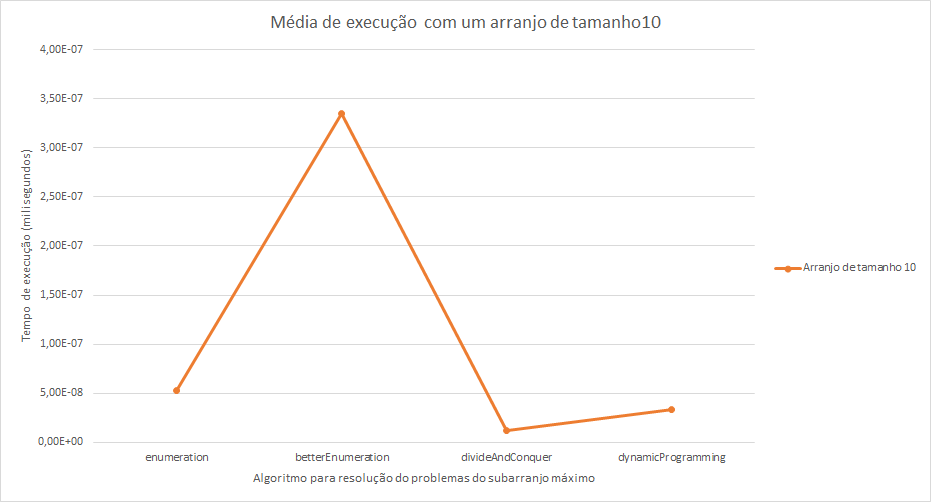
\includegraphics[width=16cm]{figuras/n=10.png}
    \caption{gráfico com a média de execução com o tamanho do arranjo sendo 10.}
    \label{fig:n=10}    
\end{figure}

\begin{figure}[!htb]
    \center
    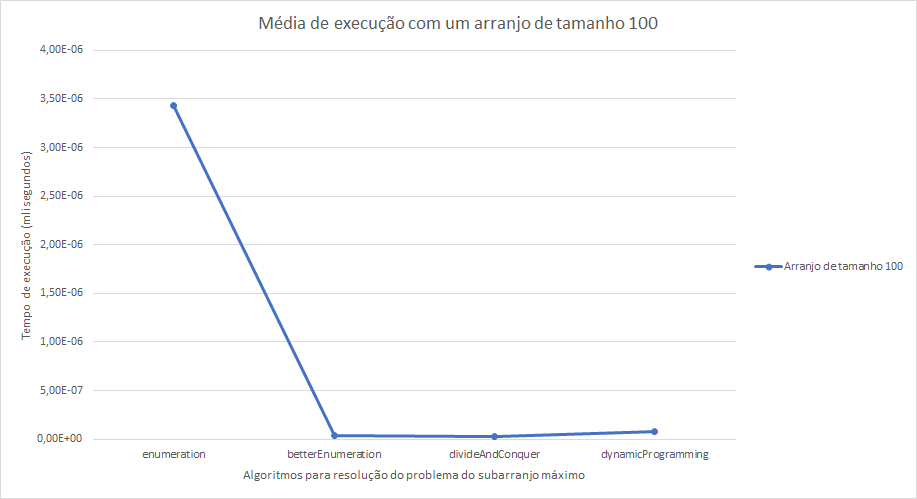
\includegraphics[width=16cm]{figuras/n=100.png}
    \caption{gráfico com a média de execução com o tamanho do arranjo sendo 100.}
    \label{fig:n=100}    
\end{figure}

\begin{figure}[!htb]
    \center
    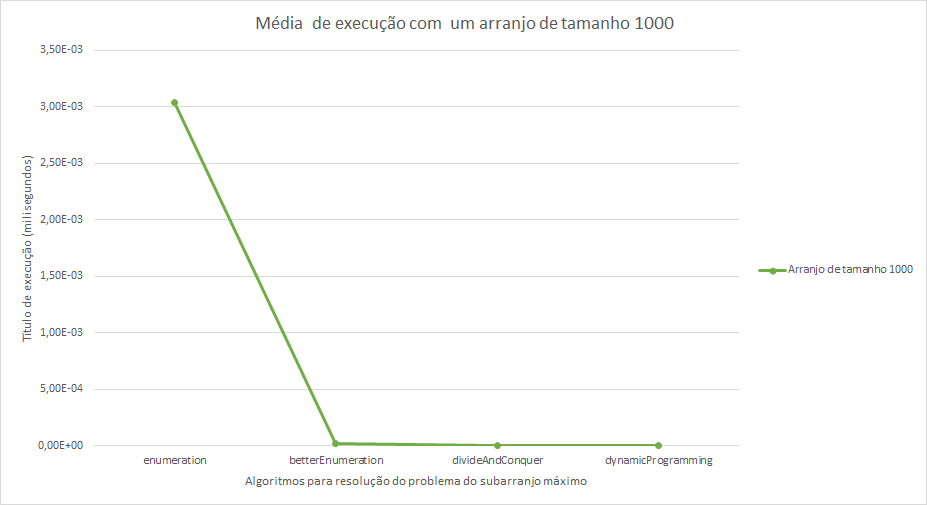
\includegraphics[width=16cm]{figuras/n=1000.png}
    \caption{gráfico com a média de execução com o tamanho do arranjo sendo 1000.}
    \label{fig:n=1000}    
\end{figure}

\begin{figure}[!htb]
    \center
    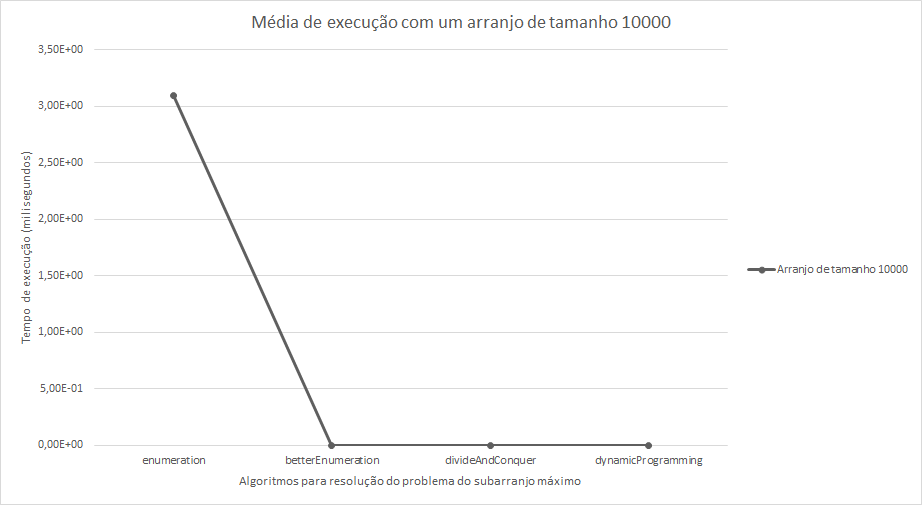
\includegraphics[width=16cm]{figuras/n=10000.png}
    \caption{gráfico com a média de execução com o tamanho do arranjo sendo 10000.}
    \label{fig:n=10000}    
\end{figure}

\clearpage
\section{Conclusões}
\label{sec:conclusoes}
Após utilizarmos a análise empírica para comparar o tempo de execução de algoritmos que procuram resolver o problema do subarranjo máximo, com tamanhos de entradas diferentes tiramos muitas lições. Uma delas é verificar as opções de algoritmos que temos para resolver um determinado problema, já que como vimos nesse problema do subarranjo máximo o algoritmo influenciam totalmente no tempo de execução de um programa. A outra lição que aprendemos com a realização desse trabalho foi que a entrada influenciam totalmente no algoritmo, já que mais iterações terão que ser feitas e o tempo de execução ficará mais elevado. Então se a nossa entrada for pequena, podemos utilizar qualquer um dos algoritmos, como podemos ver na figura \ref{fig:n=10} em que a diferença de tempo de execução não é tão grande assim. Agora se utilizarmos entradas de tamanho elevado, aí devemos considerar algoritmos de divisão e conquista ou programação dinâmica, em que há uma enorme diferença de tempo de execução, como visto na figura \ref{fig:n=10000}.

% -------------------- --------------------------------------
% ELEMENTOS PÓS-TEXTUAIS
% ----------------------------------------------------------
\postextual
% ----------------------------------------------------------
% Referências bibliográficas
% ----------------------------------------------------------
\renewcommand{\bibsection}{%
\section{\bibname}
\label{sec:referencias}
\bibmark
%\ifnobibintoc\else
%\phantomsection
%\addcontentsline{toc}{section}{\bibname}
%\fi
\prebibhook}

\bibliography{abntex2-modelo-references}

\end{document}
